% Pour guider la définition de notre méthode nous avons identifié
% plusieurs principes que nous voulons voir respectés.

\subsection{Intégration dans le contexte métier}

Le premier des principes que nous voulons voir respectés par notre
méthode est celui de sa bonne intégration dans le contexte métier.
%
C'est un point que nous avons déjà évoqué a plusieurs reprises. Nous
souhaitons que notre méthode soit conçue dans l'optique de son
application en situation réelle, c'est-à-dire que nous avons à cœur de
réfléchir à son appropriation et son utilisation par les
secouristes. Pour autant nous ne souhaitons pas sacrifier la
généricité de notre méthode, c'est pourquoi son développement relève
d'un équilibre entre la généricité de la méthode et la spécificité de
certains paramétrages.

\subsubsection{Prérequis nécessaires à la méthode de construction
  d'une zone de localisation probable}
\label{sec:4-1-1-1}

Comme nous l'avons indiqué dans la première partie, un des partis-pris
fondamentaux du projet CHOUCAS est d'intégrer pleinement les
secouristes au processus de localisation de la victime, ce qui impose
le développement de solutions d'aide à la décision et non
d'automatisation de la localisation. Si ce choix n'appose pas de
contraintes spécifiques sur nos travaux, il nous offre des
possibilités inédites. En effet, ce parti-pris impose la présence
constante d'un secouriste, en contact avec le requérant et
interagissant avec notre méthode de localisation par le biais de
l'interface développée au sein du projet Choucas
(\ref{subsec:1-2-3-3}). Par conséquent, nous pouvons développer une
méthode nécessitant la participation active d'un secouriste lors de
son application.

Nous avons donc décidé de compter sur les secouristes pour construire
les \emph{indices de localisation} à partir des informations données
par le requérant. Cette opération consiste à identifier les différents
élément constituant \emph{l'indice de localisation} (\emph{sujet,}
\emph{objet de référence,} \emph{relation de localisation}) dans le
discours du requérant, puis à les renseigner dans l'interface. Ce
travail ne se résume cependant pas à une opération de saisie mais
impose également un travail d'analyse et de désambiguïsation du
discours du requérant. Pour l'illustrer prenons l'exemple de la phrase
: \enquote{Je suis à deux pas d'une maison}. La première tâche que
nous confions au secouriste est celle de l'identification des éléments
de la phrase, \enquote{je} est le \emph{sujet,} \enquote{à deux pas}
est une \emph{relation de localisation} et \enquote{une maison} est
\emph{l'objet de référence.} Mais cette segmentation ne suffit pas à
\emph{spatialiser} cet \emph{indice de localisation.} Pour ce faire il
est nécessaire d'interpréter ces trois chaines de caractères pour
identifier l'objet ou le concept auquel elles se référent. Dans le cas
d'une automatisation intégrale il serait nécessaire de définir une
méthode à cet effet, mais nous pouvons déléguer cette tâche au
secouriste. La \emph{relation de localisation} \enquote{à deux pas}
peut, par exemple, être considérée comme une \emph{relation de
  distance (métrique) quantitative}
(cf. \ref{sec:3-1-dist_met_quant}), pourtant on peut supposer que la
notion centrale de cet exemple est la notion de \emph{proximité} et
non une quantification de distance. L'automatisation de ce travail de
désambiguïsation est extrêmement difficile et est un champ de
recherche spécifique, c'est pourquoi nous le déléguons au
secouriste. Dans les faits cela implique que c'est à ce dernier de
choisir la \emph{relation spatiale,} à partir d'une liste prédéfinie,
en fonction du contexte et de sa compréhension de \emph{l'indice de
  localisation}. Ainsi, pour reprendre l'exemple précédent, c'est au
secouriste de choisir si la \emph{relation de localisation} \enquote{à
  deux pas} doit être modélisée comme une relation de \emph{proximité}
où une \emph{distance métrique quantitative.}

De manière analogue il revient au secouriste d'analyser l'objet de
référence. Dans notre exemple, \emph{l'objet de référence}
(\enquote{une maison}) désigne un type d'objet auquel plusieurs objets
(\ie les \emph{instances}) peuvent correspondre. Ce travail
d'identification des objets géographiques utilisés comme référence par
le requérant peut également être délégué au secouriste, par le biais
de l'interface. Pour notre exemple le secouriste devra sélectionner
tous les objets correspondant à la description donnée par le
secouriste. Cette approche pose néanmoins un problème, celui de l'aire
de la sélection. En effet, sans information supplémentaire tout objet
géographique correspondant à la sélection peut être considéré comme un
objet de référence valide. Il est donc nécessaire de définir une
\emph{zone de travail} délimitant l'aire de recherche de la victime,
et par conséquent l'aire de sélection des \emph{objets de référence.}
Dans l'ontologie d'alerte CHOUCAS (OAC, \cite{Viry2019}), cette région
est qualifiée de \emph{zone initiale de recherche} \acp{zir}. La
définition d'une telle zone est un préalable indispensable à la
\emph{spatialisation} des \emph{indices de localisation.}

Ainsi, notre méthodologie impose trois tâches au secouriste. La
première, effectuée au début de la phase de localisation, consiste à
définir la \ac{zir}. La seconde consiste à identifier, à partir d'une
liste préalablement définir, \emph{la relation de localisation}
correspondant au mieux à \emph{l'indice de localisation.} La troisième
consiste à sélectionner les \emph{objets de référence} utilisés par le
requérant.
%
Ainsi, en entrée de notre méthode nous disposons, pour chaque
\emph{indice de localisation} d'une \emph{relation de localisation}
exprimée dans un vocabulaire contrôlé et d'un ensemble d'objets
géographiques servant de référence.

% \tdi{Ajout figure diag activ secours}
% \begin{figure}
%   \centering
%   % \input{../figures/diag_activ_secours.tex}
%   \caption{dcsqd}
%   \label{fig:diag_acti_secours}
% \end{figure}

\subsubsection{La modélisation explicite des connaissances}

Lorsque nous avons défini les premier éléments de note méthode de
spatialisation dans le \autoref{chap:02}, nous avons définis deux
phases, la \emph{spatialisation} et la \emph{fusion.}  Toutes deux
différent par un point essentiel. La fusion consiste à regrouper
différentes \emph{zones de localisation compatibles} dans le but de
construire une seule \emph{zone de localisation probable}
\footnote{Bien qu'elle puisse être discontinue.}, par conséquent, tous
les individus fusionnés sont du même type, des \emph{zones de
  localisation compatibles}. Une même méthode peut donc être employée
dans toutes les configurations, qu'il soit nécessaire de fusionner
deux \emph{zones de localisation} identiques ou trente \emph{zones}
extrêmement différentes. Cette généricité n'est cependant pas partagée
par la méthode de \emph{spatialisation,} qui doit avoir un
comportement adapté à la chaque \emph{relation de localisation.} En
effet, on ne peut spatialiser la \emph{relation} \enquote{sous} de la
même manière que les \emph{relations} \enquote{entre} ou
\enquote{proche}. Il est donc nécessaire de définir (et d'implémenter)
une méthode de \emph{spatialisation} chaque les \emph{relation de
  localisation} traitée. Ces différentes méthodes de
\emph{spatialisation} sont d'une grande importance. D'une part, car
elles constituent le cœur de notre travail de conception de notre
solution, c'est par elles qu'une description de position devient une
\emph{zone de localisation compatible,} de l'autre, car le
fonctionnement de ces méthodes devient \emph{de facto} un cadre
formel, fixant ---~par le biais de leur \emph{spatialisation}~--- la
sémantique que nous attribuons à chaque \emph{relation de
  localisation.} Pour le dire autrement, la meilleure façon de
comprendre comment est traitée une \emph{relation de localisation}
donnée est de consulter le code qui se destine à la
\emph{spatialiser.} Ce faisant l'ensemble des connaissances produites
lors de l'élaboration des méthodes de \emph{spatialisation} serait
principalement sous forme procédurale (\ie un algorithme \emph{ad hoc}
pour chaque méthode, implémenté par un code spécifique), ce qui est
une limite forte à la compréhension et l'utilisation appliquée de
notre travail, en plus de s'opposer au principe \emph{d'intégration
  dans le contexte métier.}

Nous avons donc cherché à séparer autant que possible la formalisation
de la sémantique des \emph{relations de localisation} de leur
implémentation, en adoptant une démarche de modélisation explicite des
connaissances, librement inspirée des \emph{systèmes à base de
  connaissances} \autocite{LeBer2006}. Dans ces systèmes, les
connaissances sont formalisées sous forme déclarative au sein d'une
ontologie lue et interprétée par un logiciel, dont le comportement est
défini une fois pour toutes mais est guidé par ces connaissances. On
peut donc imaginer que les règles de \emph{spatialisation} de toutes
les \emph{relations de localisations} soient formalisées dans une
ontologie \emph{ad hoc} et interprétées et appliquées par un logiciel
spécifique, dédié au traitement des connaissances contenues dans cette
ontologie. Cette approche a de multiples avantages. D'une part, elle
permet aux utilisateurs des méthodes de \emph{spatialisation} de
disposer d'une forme d'auto-documentation, permise par la
centralisation de toutes les règles de \emph{spatialisation.} De plus,
cette centralisation facilite également la modification ou l'ajout de
règles de \emph{spatialisation,} faisant de l'ontologie un outil
facilitant l'amélioration des méthodes de \emph{spatialisation.}
Enfin, le cadre formel et la centralisation offerts par l’utilisation
d'une ontologie facilitent la diffusion de notre travail, un tel
document pouvant être plus facilement étudié, voire réutilisé, qu'un
code informatique, même diffusé librement.

\subsection{Principes de modélisation}

\subsubsection{Décomposition des \emph{relations de localisation}}
\label{subsec:4-1-2-1}

Comme nous l'avons déjà indiqué (\autoref{subsec:2-1-1}), une même
\emph{relation de localisation} peut avoir une sémantique différente
en fonction de son contexte d'utilisation
\autocite[16]{Borillo1998}. Par exemple, la \emph{relation de
  localisation} \enquote{\emph{sous}} n'a pas exactement la même
signification dans les phrases : \enquote{Je suis sous \emph{un pont}}
et \enquote{Je suis sous \emph{une route}}. La première phrase
sous-entend une idée de \emph{recouvrement} (\ie \emph{le pont est
  entre le locuteur et le ciel}), que l'on retrouve également dans
l'expression imagée \enquote{Je suis sous l'eau}, mais cette notion
est absente dans la seconde phrase, qui décrit une configuration où le
recouvrement est impossible \footnote{Du moins en contexte
  montagneux.}. Il est intéressant de noter l'intuitivité
\footnote{Dans la mesure où l'on est un locuteur humain.} de cette
distinction. De fait, on comprend immédiatement que la phrase
\enquote{Je suis sous un pont} décrit une configuration plus précise
qu'une simple différence d'altitude et, à l'inverse, on ne peut
imaginer que la phrase : \enquote{Je suis sous une route} décrive une
situation où le locuteur est littéralement recouvert par la
voirie. Cette interprétation différente de deux phrases très
similaires ne s'explique que par leur point divergent, leur
\emph{objet de référence} et plus particulièrement, leur nature. On
peut, en effet, être recouvert par \emph{un pont} (ou un arbre, une
table, le ciel, \emph{etc.}) mais pas par une route (ou un
glacier). \emph{L'objet de référence} et plus généralement le contexte
d'utilisation d'une \emph{relation de localisation,} peut donc influer
sur sa signification. Dès lors, on ne peut prétendre spatialiser des
\emph{relations de localisation} sans être capable d'identifier ces
variations de sémantique, leurs causes et leurs conséquences.

Pour aborder ce problème, nous postulons que la différence sémantique
de ces deux exemples s'explique en réalité par l’emploi de deux
\emph{relations de localisations} différentes, mais désignées par la
même \emph{préposition spatiale :} \enquote{sous}. Adopter cette
vision implique donc de considérer que le \enquote{sous} \emph{avec
  recouvrement} est une \emph{relation de localisation} différente du
\enquote{sous} \emph{sans recouvrement} et ce bien qu'elles soient
exprimées avec la même \emph{préposition spatiale.} Nous adoptons ce
postulat en le généralisant à l'ensemble du vocabulaire. De la même
manière, on pourrait considérer que les différentes définitions d'un
même mot, que l'on peut trouver dans un dictionnaire, définissent des
concepts différents, mais exprimés avec le même mot. Cette conception
a beau présenter un certain intérêt intellectuel, nous pensons qu'elle
ne suffit pas à apporter une solution. D'autre part elle ne dispense
pas du travail d’identification des variantes des \emph{relations de
  localisation,} mais quelle approche le pourrait ?  D'autre part,
elle ignore un élément important que nous n'avons pas encore mentionné
: les \emph{récurrences sémantiques.} Si le \enquote{sous} avec et
sans recouvrement s'opposent, ils partagent une part importante de
leur sémantique, ce qui leur vaut d'être désignés avec la même
préposition. Ces deux \emph{relations spatiales} traduisent toutes
deux une situation ou le \emph{sujet} a une altitude inférieure à
\emph{l'objet de référence} et où ces deux éléments ne sont pas très
éloignés. La notion de recouvrement ne fait que s'ajouter à ces deux
notions. Aussi, ces deux \enquote{sous} ont plus de points communs que
de points de divergence. On observe donc la présence de
\emph{récurrences sémantiques} entre ces deux \emph{relations.} Nous
proposons de tirer parti de ces récurrences pour améliorer notre
précédent postulat. Ainsi, nous considérons que les deux variantes du
\enquote{sous} sont des \emph{relations de localisation} différentes
car elles combinent des \enquote{briques sémantiques} différentes,
tout en en partageant la plupart. L’intérêt majeur de ce point de vue
est qu'il laisse entrevoir la possibilité d'exploiter ces récurrences
sémantiques pour la \emph{spatialisation} \autocite{Bunel2019a}. Pour
ce faire, nous proposons \enquote{d'extraire}, lors d'un processus que
nous appelons \emph{décomposition,} ces \enquote{briques sémantiques}
des \emph{relations de localisation,} pour définir un ensemble de
\emph{relations de localisation} que nous appelons \emph{atomiques,}
qui, combinées, recréent la sémantique de la \emph{relation de
  localisation} décomposée. La mise en place de cette approche
nécessite l'identification et l'explicitation préalables des
\emph{relations de localisation atomiques,} conformément au
\emph{principe de modélisation explicite des connaissances.} Chaque
relation de \emph{localisation atomique} correspondant alors à une
composante sémantique indépendante.

Pour illustrer cette démarche on peut l'appliquer à \emph{l'indice de
  localisation} : \enquote{Je suis sous une route}. Comme nous l'avons
mentionné, la \emph{relation de localisation} utilisée décrit ici une
situation où le locuteur est situé à une altitude inférieure d'une
route donnée, mais également a proximité de cette dernière, de sorte
que la relation de verticalité entre le locuteur et la route soit
saillante \autocite{Vandeloise1986}. La relation de localisation
\enquote{sous} peut ici être décomposée en deux \emph{relations de
  localisation atomiques,} la première indiquant que le \emph{sujet}
est situé plus bas que \emph{l'objet de référence} et la seconde
indiquant qu'il en est proche.

La \emph{décomposition} d'une \emph{relation de localisation} peut
être envisagée comme une opération permettant de construire de
nouveaux \emph{indices de localisation} à partir d'un \emph{indice}
initial utilisant une \emph{relation de localisation} non
atomique. Les \emph{indices de localisation} dérivés ne diffèrent que
par leur \emph{relation de localisation} (\ie qu'ils partagent
\emph{leur sujet,} \emph{leur relation de localisation} et leur
\emph{objet de référence}). En créant de nouveaux \emph{indices de
  localisation,} la \emph{décomposition} permet de les
\emph{spatialiser} indépendamment. On peut alors \emph{spatialiser}
\emph{l'indice de localisation} initial en combinant les \emph{zones
  de localisation compatibles} résultant de la \emph{spatialisations}
des \emph{relations de localisations atomiques.} Ainsi, pour
\emph{spatialiser} l'\emph{indice de localisation} \enquote{je
  \emph{suis sous} une route}, nous construisons la \emph{zone de
  localisation} correspondant à \emph{l'indice de localisation}
\enquote{je suis \emph{proche} d'une route} et la \emph{zone de
  localisation} correspondant à \emph{l'indice de localisation}
\enquote{je suis \emph{à une altitude inférieure} à une route,} puis
nous les combinons à l'aide d'un opérateur \emph{ad hoc,} permettant
d'obtenir la \emph{zone de localisation compatible} correspondant à
\emph{l'indice de localisation} \enquote{je suis \emph{sous} une
  route}.

Cette approche fondée sur la \emph{décomposition} n'est pas limitée
aux \emph{relations de localisation} dérivées d'une notion plus large
(\eg le \enquote{sous} avec recouvrement qui dérive du \enquote{sous}
au sens large). D'autres \emph{récurrences sémantiques} peuvent
apparaitre dans des \emph{relations de localisation} très
différentes. La notion de \emph{proximité,} déjà utilisée, est, par
exemple, à la base de nombreuses autres \emph{relations de
  localisation} comme \enquote{\emph{à côté}}, \enquote{\emph{aux
    alentours de}}, \enquote{\emph{devant}}, \emph{etc.} En
définissant une méthode de \emph{spatialisation} de cette
\emph{relation de localisation atomique} il devient possible de la
réutiliser et de la combiner à d'autres \emph{relations de
  localisation atomiques} permettant ainsi de modéliser un grand
ensemble de \emph{relations de localisations.}

Les différents exemples présentés ici ne doivent cependant pas faire
croire que les \emph{relations de localisation} sont systématiquement
décomposables. La notion de proximité, par exemple, peut être utilisée
lors de décompositions, mais elle est également pertinente en
elle-même, comme dans \emph{l'indice de localisation} : \enquote{Je
  suis proche d'une route}. Certaines des \emph{relations de
  localisation} manipulées par les requérants peuvent donc s’avérer
être \emph{atomiques.} Cette observation ne remet pas en cause cette
approche, mais elle montre que la \emph{décomposition} n'est pas une
étape systématique.

%\tdi{Ajouter le principe de décomposition des objets ?}

\subsubsection{Autonomie de la \emph{spatialisation}}

Dans le \autoref{chap:02} nous avons indiqué que la création d'une
\emph{zone de localisation probable} à partir d'un ensemble
\emph{d'indices de localisation} nécessitait deux étapes successives:
% 
\begin{enumerate*}[label=(\alph*)]
\item la \emph{spatialisation} des \emph{indices de localisation} et
\item la \emph{fusion} des \emph{zones de localisation compatibles} en
résultant.
\end{enumerate*}
% 
Bien que ces deux étapes soient indispensables, elles peuvent être
combinées de différentes manières. Une première solution, illustrée
par la figure \ref{fig:comp_approches_lin}, consiste à
\enquote{chainer} les \emph{spatialisations,} de manière à ce que la
\emph{zone de localisation compatible} résultant de la
\emph{spatialisation} d'un \emph{indice} soit la \emph{zone initiale
  de recherche} du \emph{second indice de localisation.} Cette
approche pourrait être qualifiée de soustractive, dans la mesure où
les positions n'appartenant par à la \emph{zone de localisation
  probable} sont retirées au fur et à mesure des
\emph{spatialisations,} jusqu'à l'obtention de la \ac{zlp}. Les
différentes \emph{zones de localisation compatibles} sont donc créées
les unes à la suite des autres, ce qui a pour effet de lier
implicitement les résultats des différentes \emph{spatialisations.}
Avec cette approche, l'opération de \emph{fusion} est implicite: elle
s'opère en partie à chaque nouvelle \emph{spatialisation,} puisque les
zones ne correspondant pas aux \emph{indices de localisation} sont
retirées peu à peu. La \emph{zone de localisation probable} (en bleu
sur la figure \ref{fig:comp_approches}) est obtenue une fois que l'on
a \emph{spatialisé} tous les \emph{indices de localisation.} Cette
approche à l'avantage d'être simple à concevoir et à développer, mais
elle a un défaut majeur : la propagation des erreurs. À cause de
l'enchainement des étapes de \emph{spatialisation,} les potentielles
erreurs de \emph{spatialisation} peuvent modifier le résultat des
\emph{spatialisations} ultérieures. Imaginons par exemple que l'on
souhaite construire la \ac{zlp} correspondant à \emph{l'indice de
  localisation} : \enquote{Je suis dans une forêt, près du refuge.} Si
l'on décide de commencer par \emph{spatialiser} \emph{l'indice de
  localisation} : \enquote{Je suis dans une forêt} on obtiendra une
\emph{zone de localisation compatible} (qui correspond à la seconde
étape de la figure \ref{fig:comp_approches_lin}) réduisant l'aire de
recherche. La \emph{spatialisation} du second \emph{indice de
  localisation} consistera donc à chercher les positions qui
correspondent à \emph{l'indice de localisation} \enquote{Je suis
  proche du refuge} dans cette zone réduite (\ie la troisième étape du
la figure \ref{fig:comp_approches_lin}). Le problème de la
répercussion des erreurs se pose si le résultat de la première
\emph{spatialisation} est faux, (\eg une des forêts pouvant faire
office \emph{d'objet de référence} n'est pas prise en compte). Deux
cas de figure sont alors possibles : soit la \emph{zone de
  localisation} résultant de la \emph{spatialisation} est trop étendue
\footnote{C'est-à-dire que certaines de positions retenues sont de
  faux positifs.}, soit trop réduite \footnote{C'est-à-dire que
  certaines de positions retenues sont de faux
  négatifs.}\multiplefootnoteseparator \footnote{Ce qui est, par
  exemple, le résultat de l'oubli d'un \emph{objet de référence.}}.
Dans le premier cas, la \emph{spatialisation} du second \emph{indice
  de localisation} sera effectuée dans une zone plus étendue que
nécessaire, ce qui peut avoir pour effet de produire une \emph{zone de
  localisation probable} contenant des positions erronées. Le second
cas est plus problématique, puisque la \emph{spatialisation} du second
\emph{indice de localisation} est effectuée à partir d'une zone trop
réduite, des positions devant appartenir à la \emph{zone de
  localisation probable} pourront donc être ignorées, dont la position
de victime\footnote{Ces deux cas de figure correspondent à des
  erreurs, respectivement, de type II et I.}. Ainsi, si un des
\emph{indices de localisation} est mal \emph{spatialisé}, que ce soit
à cause de la méthode utilisée ou d'une mauvaise description, cela se
répercute sur toutes les \emph{spatialisations} ultérieures et la
moindre correction impose donc de refaire l'ensemble des traitements.

Une seconde solution, plus robuste, est cependant permise par une des
caractéristiques des \emph{indices de localisation,} leur
indépendance. Il n'est, en effet, généralement pas nécessaire de
connaitre le résultat de la \emph{spatialisation} d'un \emph{indice de
  localisation} pour pouvoir \emph{spatialiser} les autres
\emph{indices} d'une même alerte. Par exemple, la description
précédemment utilisée : \enquote{Je suis dans une forêt, près du
  refuge}, contient deux \emph{indices de localisation,} qui,
regroupés participent à décrire une même position. Mais ces deux
\emph{indices} conservent leur sens s'ils sont énoncés
séparément. Dire, \enquote{Je suis dans une forêt} ou \enquote{je suis
  près du refuge} est une description valide, même si moins précise
que \emph{l'indice de localisation} initial. Cette indépendance des
\emph{indices} permet de mettre en place une \emph{spatialisation}
parallèle, comme le montre la figure
\ref{fig:comp_approches_sep}. Avec cette approche la
\emph{spatialisation} des différents \emph{indices de localisation}
est effectuée séparément et leur \emph{fusion} est effectuée dans un
second temps. Comme pour la démarche \enquote{chainée} une
\emph{spatialisation} erronée peut impacter la \emph{zone de
  localisation probable,} toutefois il est plus facile de corriger ces
erreurs. En effet, si les différentes \emph{zones de localisation
  compatibles} ont été conservées il est possible de faire une
nouvelle \emph{fusion} en retirant un, ou plusieurs \emph{indices de
  localisation.} Alors qu'avec une approche \enquote{chainée} il est
nécessaire de refaire toutes les opérations de \emph{spatialisations}
ultérieures à celle de \emph{l'indice de localisation} que l'on
souhaite modifier ou retirer et ce même si les résultats
intermédiaires ont été conservés.

\begin{figure}
  \centering
  \subfloat[Construction suivant une démarche linéaire]{
    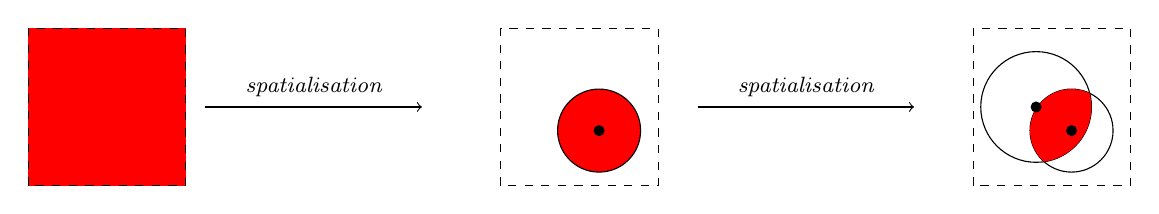
\begin{tikzpicture}

  \begin{scope}
    \path[fill=red] (0,0) rectangle (2,2);
	\path[draw, dashed] (0,0) rectangle (2,2);
  \end{scope}

  \path[draw, ->] (2.25,1) --++ (2.75,0)  node[pos=.5, above] {\footnotesize \itshape spatialisation};

  \begin{scope}[xshift=6cm]
	\path[draw, dashed] (0,0) rectangle (2,2);
	\begin{scope}
	    \begin{scope}
	      \clip (0,0) rectangle (2,2);
	      \fill[red] (1.25,.7) circle [radius=15pt];
	      \path[draw] (1.25,.7) circle [radius=15pt];
	    \end{scope}
	\end{scope}
    \node[circle, inner sep=0pt,minimum size=4pt, fill] (c) at (1.25,.7)
    {};
  \end{scope}



  \path[draw, ->] (8.5,1) --++ (2.75,0)  node[pos=.5, above] {\footnotesize \itshape spatialisation};




  \begin{scope}[xshift=12cm]
	\path[draw, dashed] (0,0) rectangle (2,2);
	\path[draw] (1.25,.7) circle [radius=15pt];
    \path[draw](.8,1) circle [radius=20pt];
	\begin{scope}
	    \begin{scope}
	      \clip (1.25,.7) circle [radius=15pt];
	      \fill[red] (.8,1) circle [radius=20pt];
	    \end{scope}
	\end{scope}
    \node[circle, inner sep=0pt,minimum size=4pt, fill] (c) at (1.25,.7)
    {};
    \node[circle, inner sep=0pt,minimum size=4pt, fill] (c) at (.8,1)
    {};
  \end{scope}


\end{tikzpicture}
    \label{fig:comp_approches_lin}
  }

  \subfloat[Construction suivant une démarche autonome]{
    \begin{tikzpicture}

  \begin{scope}
    \path[ffa] (0,0) rectangle (2,2);
    \path[ffc] (0,0) rectangle (2,2);
  \end{scope}

  \path[draw, ->] (2.25,1) --++ (2.75,1.5)  node[pos=.5, above] {\footnotesize \itshape spatialisation};
  \path[draw, ->] (2.25,1) --++ (2.75,-1.5)  node[pos=.5, above] {\footnotesize \itshape spatialisation};

  \begin{scope}[xshift=6cm, yshift=-1.5cm]
    \path[draw, dashed] (0,0) rectangle (2,2);
    \begin{scope}
      \begin{scope}
        \clip (0,0) rectangle (2,2);
        \fill[ffa] (1.25,.7) circle [radius=15pt];
        \path[ffc] (1.25,.7) circle [radius=15pt];
      \end{scope}
    \end{scope}
    \node[circle, inner sep=0pt,minimum size=4pt, fill] (c) at (1.25,.7)
    {};
  \end{scope}

  \begin{scope}[xshift=6cm,yshift=1.5cm]
    \path[draw, dashed] (0,0) rectangle (2,2);
    \fill[ffa](.8,1) circle [radius=20pt];
    \path[ffc](.8,1) circle [radius=20pt];
    \node[circle, inner sep=0pt,minimum size=4pt, fill] (c) at (.8,1)
    {};
  \end{scope}

  \path[draw, ->] (8.5,1) --++ (2.75,0)  node[pos=.5, above] {\footnotesize \itshape fusion};


  \begin{scope}[xshift=12cm]
    \path[draw,dashed] (0,0) rectangle (2,2);
    \path[draw,dashed] (1.25,.7) circle [radius=15pt];
    \path[draw,dashed](.8,1) circle [radius=20pt];
    \begin{scope}
      \begin{scope}
        \clip (1.25,.7) circle [radius=15pt];
        \fill[ffa2] (.8,1) circle [radius=20pt];
        \path[ffc2] (.8,1) circle [radius=20pt];
      \end{scope}
      \begin{scope}
        \clip (.8,1) circle [radius=20pt];
        \path[ffc2] (1.25,.7) circle [radius=15pt];
      \end{scope}
    \end{scope}
    \node[circle, inner sep=0pt,minimum size=4pt, fill] (c) at (1.25,.7)
    {};
    \node[circle, inner sep=0pt,minimum size=4pt, fill] (c) at (.8,1)
    {};
  \end{scope}


\end{tikzpicture}
    \label{fig:comp_approches_sep}
  }
  \caption{Comparaison du processus de construction de la \emph{zone
      de localisation probable} pour une alerte à deux \emph{indices
      de localisation}.}
  \label{fig:comp_approches}
\end{figure}

Ce principe de \emph{spatialisation} autonome n'est pas cantonné aux
\emph{indices de localisation.} Comme nous l'avons illustré
précédemment, certaines \emph{relations de localisation} peuvent être
décomposées en des \emph{relations de localisation atomiques.} Ce
processus permet de construire des nouveaux \emph{indices de
  localisation} à partir de \emph{l'indice} initial. Ces nouveaux
\emph{indices} conservent la propriété d'indépendance, puisque les
\emph{relations de localisation atomiques} décrivent des concepts
sémantiquement orthogonaux. Le principe de modélisation autonome peut
donc être étendu aux \emph{indices de localisation} décomposés, ce qui
le rend d'autant plus pertinent.

\subsubsection{Le raisonnement logique en monde ouvert}

Le dernier des principes de modélisation que nous souhaitons fixer est
celui du raisonnement en \emph{monde ouvert}. Ce terme, issu du monde
de la logique formelle, désigne un cadre de raisonnement où l'on ne
considère que l'ignorance ou l'indémontrabilité d'une règle logique
n'implique pas sa fausseté, par opposition à l'hypothèse du
\emph{monde clos.} La \autoref{fig:comp_md} tente d'illustrer ces deux
hypothèses opposées. L'ensemble de toutes les assertions logiques est
réparti entre deux ensembles, celui des assertions vraies et celui
assertions fausses. Parmi toutes ces assertions seules certaines
d'entre-elles nous sont connues \footnote{Où sont démontrables en un
  temps fini}, elles forment un nouvel ensemble plus réduit, mais
pouvant contenir des assertions vraies ou fausses, d'où
l'intersections de ces ensembles sur les deux figures. La différence
entre la figure \ref{fig:md_ferme}, représentant l'hypothèse du
\emph{monde clos} et la figure \ref{fig:md_ouvert}, représentant
l'hypothèse du \emph{monde ouvert}, réside dans la manière dont sont
représentées les assertions inconnues, c'est-à-dire en dehors de
l'ensemble des règles connues. Dans le premier cas elles ne peuvent
être situées que dans l'ensemble des assertions fausses, car
l'ensemble des assertions vraies est intégralement contenu dans
l'ensemble des règles connues. Alors que dans la figure représentant
l'hypothèse du \emph{monde ouvert} les assertions n'appartenant par à
l'ensemble des assertions connues peuvent être dans l'ensemble des
règles vraies ou des règles fausses. Ainsi, dans \emph{l'hypothèse du
  monde clos} (figure \ref{fig:md_ferme}) toute règle inconnue est
considérée comme fausse. Alors que dans \emph{l'hypothèse du monde
  ouvert} (Figure \ref{fig:md_ouvert}) les règles inconnues sont
considérées comme telles, \ie que l'on estime qu'elles peuvent être
vraies, comme fausses.

Pour illustrer la différence entre ces deux hypothèses on peut prendre
l'exemple suivant. Imaginons que je décrive le contenu de ma
bibliothèque de la manière suivante : \enquote{Dans ma bibliothèque on
  trouve les ouvrages : \emph{méthodes de logique,} de Willard
  \bsc{Quine} et \emph{le projet \emph{Cybersyn},} d'Eden
  \bsc{Medina}.} Cette phrase peut être décomposée en deux assertions
logiques, \enquote{ma bibliothèque contient l'ouvrage \emph{méthodes
    de logique}} et \enquote{ma bibliothèque contient l'ouvrage
  \emph{le projet \emph{Cybersyn}}.} Avec \emph{l'hypothèse du monde
  clos} toute autre proposition logique est considérée comme fausse,
comme l'illustre la figure \ref{fig:md_ferme}. Ainsi à la question
\enquote{Est-ce que tu as \emph{l'espace en français,} de Claude
  \bsc{Vandeloise} ?} ---~ou tout autre livre~--- la réponse sera
\enquote{non}. Cela revient à considérer que j'ai donné une
description exhaustive du contenu de ma bibliothèque. Si l'on fait
\emph{l'hypothèse d'un monde ouvert} on considère que les règles qui
nous sont inconnues peuvent être vraies ou fausses (figure
\ref{fig:md_ouvert}). Ainsi, dans ce cadre on ne peut que répondre
\enquote{Je ne sais pas} à la question précédente. Dans
\emph{l'hypothèse d'un monde ouvert,} l’absence d'une règle n'implique
pas sa fausseté.

\begin{figure}
  \centering
  \subfloat[]{
    \begin{tikzpicture}
  \begin{scope}
    \fill[ffa] (1,.75) arc(90:270:.75) -- cycle;% [radius=.75cm];
    \path[ffc] (1,.75) arc(90:270:.75) -- cycle;
    \node[color=RdBu-9-1] at (.625,0) {V};
  \end{scope}
  \begin{scope}
    \fill[ffa2] (1,1) arc(270:90:-1) -- cycle;% [radius=.75cm];
    \path[ffc2] (1,1) arc(270:90:-1) -- cycle;
    \node[color=RdBu-9-9] at (1.375,0) {F};
  \end{scope}
  \begin{scope}
    \path[ffc, draw=black] (1,0) circle [radius=.75cm];
  \end{scope}
  \begin{scope}
    \node (rect) [anchor=north, minimum width=.5cm,minimum
    height=.25cm,ffc, draw=black] at (0,-1.25) {};
    \node[anchor=west, font=\tiny\vphantom{Ag}, text width = 4cm] at
    ([xshift=1ex]rect.east) {Connues};
    
    \node (rect2) [anchor=north, minimum width=.5cm,minimum
    height=.25cm, ffa, ffc] at ([yshift=-.25cm]rect) {};
    \node[anchor=west, font=\tiny\vphantom{Ag}, text width = 4cm] at
    ([xshift=1ex]rect2.east) {Vraies};
    
    \node (rect3) [anchor=north, minimum width=.5cm,minimum
    height=.25cm, ffa2, ffc2] at ([yshift=-.25cm]rect2) {};
    \node[anchor=west, font=\tiny\vphantom{Ag}, text width = 4cm] at
    ([xshift=1ex]rect3.east) {Fausses};
    
    \draw[decorate,decoration={brace}] ([xshift=7.75ex]rect.north
    east) -- ([xshift=7.75ex]rect3.south east);
    \node[anchor=west, font=\tiny\vphantom{Ag}, text width = 2cm] at
    ([xshift=8ex]rect2.east) {Ensemble des règles};   
  \end{scope}
\end{tikzpicture}
    \label{fig:md_ferme}
  }\hspace{2cm}
  \subfloat[]{
    \begin{tikzpicture}
  \begin{scope}
    \fill[ffa] (1,1) arc(90:270:1) -- cycle;% [radius=.75cm];
    \path[ffc] (1,1) arc(90:270:1) -- cycle;
    \node[color=RdBu-9-1] at (.625,0) {V};
  \end{scope}
  \begin{scope}
    \fill[ffa2] (1,1) arc(270:90:-1) -- cycle;% [radius=.75cm];
    \path[ffc2] (1,1) arc(270:90:-1) -- cycle;
    \node[color=RdBu-9-9] at (1.375,0) {F};
  \end{scope}
  \begin{scope}
    \path[ffc, draw=black] (1,0) circle [radius=.75cm];
    \node[text width=3cm] (leg) at (4,1)
    {\footnotesize \itshape Ensemble des règles connues};
    \path[draw, ->] (leg.west) --++ (25:-.9);
  \end{scope}
\end{tikzpicture}
    \label{fig:md_ouvert}
  }
  \caption{Illustration des hypothèses du \emph{monde clos}
    \protect\subref{fig:md_ferme} et du \emph{monde ouvert}
    \protect\subref{fig:md_ferme}}
  \label{fig:comp_md}
\end{figure}

Appliqué à notre cas d'étude le choix d'une de ces deux hypothèses
revient à se demander si la description d'une position donnée par les
requérants est systématiquement exhaustive. Si la réponse est
\enquote{oui} on peut alors faire \emph{l'hypothèse d'un monde clos}
et considérer que toute information qui n'est pas donnée par le
requérant est fausse. Ainsi, s'il décrit sa position en indiquant
qu'il \enquote{est sur une route} on pourra en conclure qu'il est pas
en forêt, puisque cette information ne nous a pas été donnée. Par
conséquent on pourra \emph{spatialiser} cette alerte à l'aide de deux
\emph{indices de localisation} l'un explicite (\enquote{je suis sur
  une route}) et l'autre inféré (\enquote{je ne suis pas en
  forêt}). Or cet exemple illustre bien que cette approche n'est pas
satisfaisante, des routes peuvent traverser des forêts, ou non et rien
dans cette alerte ne permet de rejeter cette hypothèse, le
raisonnement en monde ouvert est donc plus approprié.

%%% Local Variables:
%%% mode: latex
%%% TeX-master: "../../../../main"
%%% End:
